\documentclass[tikz,border=10pt]{standalone}
\usetikzlibrary{arrows.meta, calc}
\usepackage{amsmath} % Required for \text{}

\begin{document}
	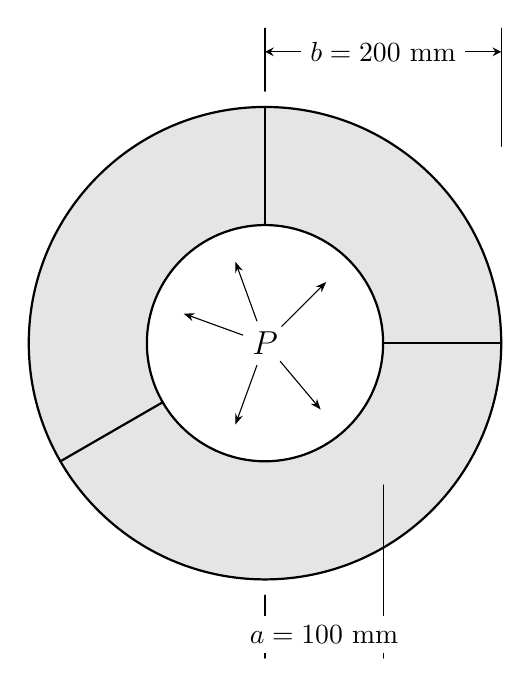
\begin{tikzpicture}[line join=round, line cap=round]
		
		% Parameters
		\def\rI{1.5} % Inner radius a
		\def\rO{3.0} % Outer radius b
		
		% 1. Draw the gray cross-section (the "meat" of the shell)
		% This fills the area between circles in the visible quadrant
		\fill[gray!20] (0,0) circle (\rO);
		\fill[white] (0,0) circle (\rI);
		
		% 2. Draw the 'cutout' lines to simulate the 3D perspective
		\draw[thick] (0, \rI) -- (0, \rO);
		\draw[thick] (\rI, 0) -- (\rO, 0);
		\draw[thick] (210:\rI) -- (210:\rO);
		
		% Arcs for the inner cavity edges
		\draw[thick] (0, \rI) arc (90:0:\rI);
		\draw[thick] (0, \rI) arc (90:210:\rI);
		\draw[thick] (\rI, 0) arc (0:-150:\rI);
		
		% 3. Outer boundary and hidden lines
		\draw[thick] (0,0) circle (\rO);
		\draw[dashed, thin] (0,0) circle (\rI);
		
		% 4. Pressure P and arrows
		\node at (0,0) {\large $P$};
		\foreach \angle in {45, 110, 160, 250, 310} {
			\draw[-{Stealth[scale=0.8]}] (\angle:0.3) -- (\angle:1.1);
		}
		
		% 5. Dimensions (using math mode without \text if you prefer to avoid packages)
		% Dimension b
		\draw (0, \rO + 0.2) -- (0, \rO + 1.0);
		\draw (\rO, \rO - 0.5) -- (\rO, \rO + 1.0);
		\draw[<->, >=stealth] (0, \rO + 0.7) -- (\rO, \rO + 0.7) 
		node[midway, fill=white] {$b = 200 \text{ mm}$};
		
		% Dimension a
		\draw (0, -\rO - 0.2) -- (0, -\rO - 1.0);
		\draw (\rI, -\rO + 1.2) -- (\rI, -\rO - 1.0);
		\draw[<->, >=stealth] (0, -\rO - 0.7) -- (\rI, -\rO - 0.7) 
		node[midway, fill=white] {$a = 100 \text{ mm}$};
		
	\end{tikzpicture}
\end{document}